\chapter{Исследование физических характеристик детектора <<Лазерного поляриметра>>}
\section{Определение уровня шумов детектора}
\label{sec:noise_study}
\begin{figure}[H]
	\begin{center}
		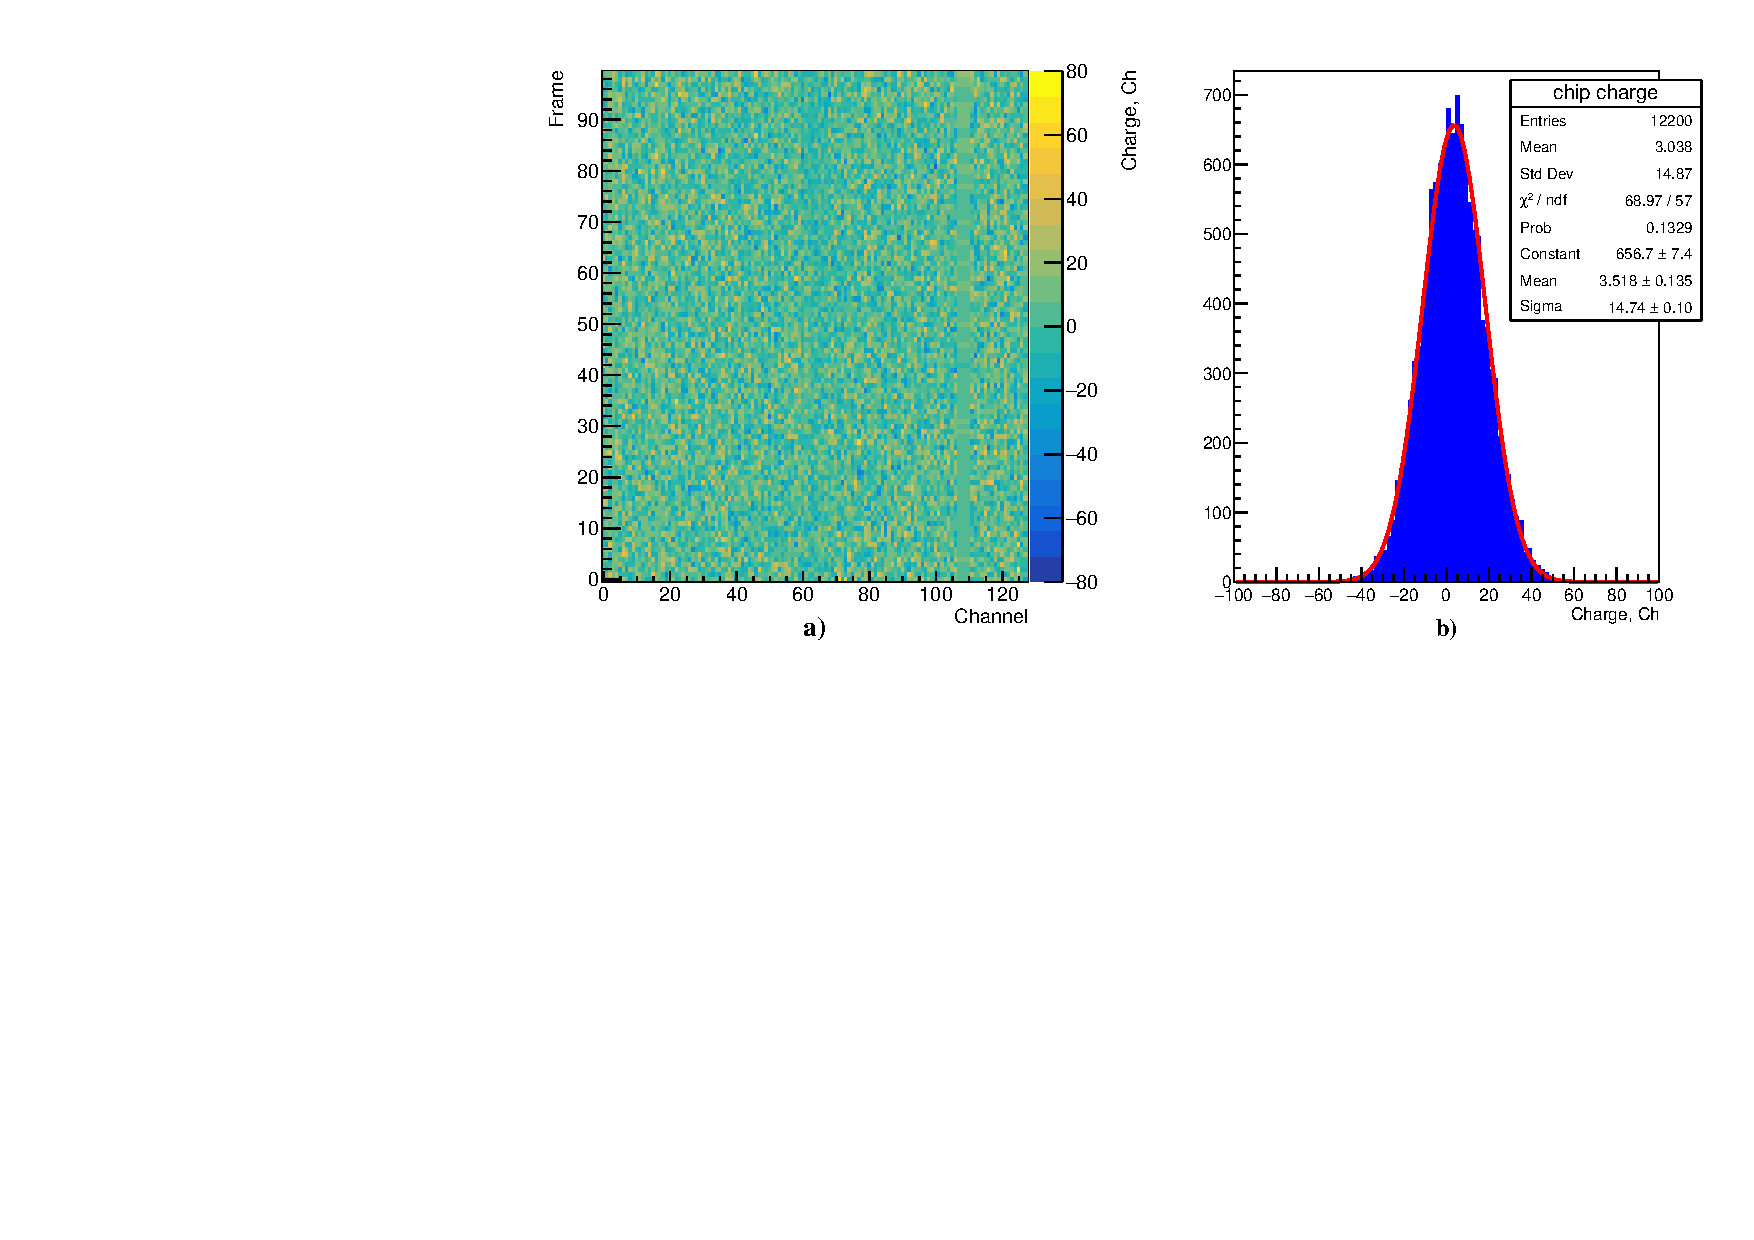
\includegraphics[width = 12cm, height = 6cm]{img/noise_map.pdf}
		\caption{a): Вид шумового события после вычитания пьедестала b): Распределение заряда в шумовом событии}
		\label{noise_map}
	\end{center}
\end{figure}
Рис. \ref{noise_map} показывает вид одного шумового события и распределение заряда в кадрах и каналах. Важным значением, которое можно извлечь уже из одного шумового события является уровень шумов. Его можно определить как корень из дисперсии распределения на Рис. \ref{noise_map} b). Шумы в данном эксперименте составили $\approx15$ каналов АЦП. Если взять несколько шумовых событий, то можно уточнить данное значение. Более того, записывая данные через равные промежутки времени, можно зафиксировать наличие дрейфа уровня шумов и их среднего значения. Такое исследование тоже было проведено. Для каждого набора данных существовала привязка по времени начала измерения. Чтобы определить, временной дрейф уровня среднего значения шумов, нами были Его результаты показали, что уровень шумов со временем меняется незначительно (Рис.\ref{fig:Noise_gr}.)

\begin{figure}[h]
	\centering
	\begin{subfigure}{.5\textwidth}
		\centering
		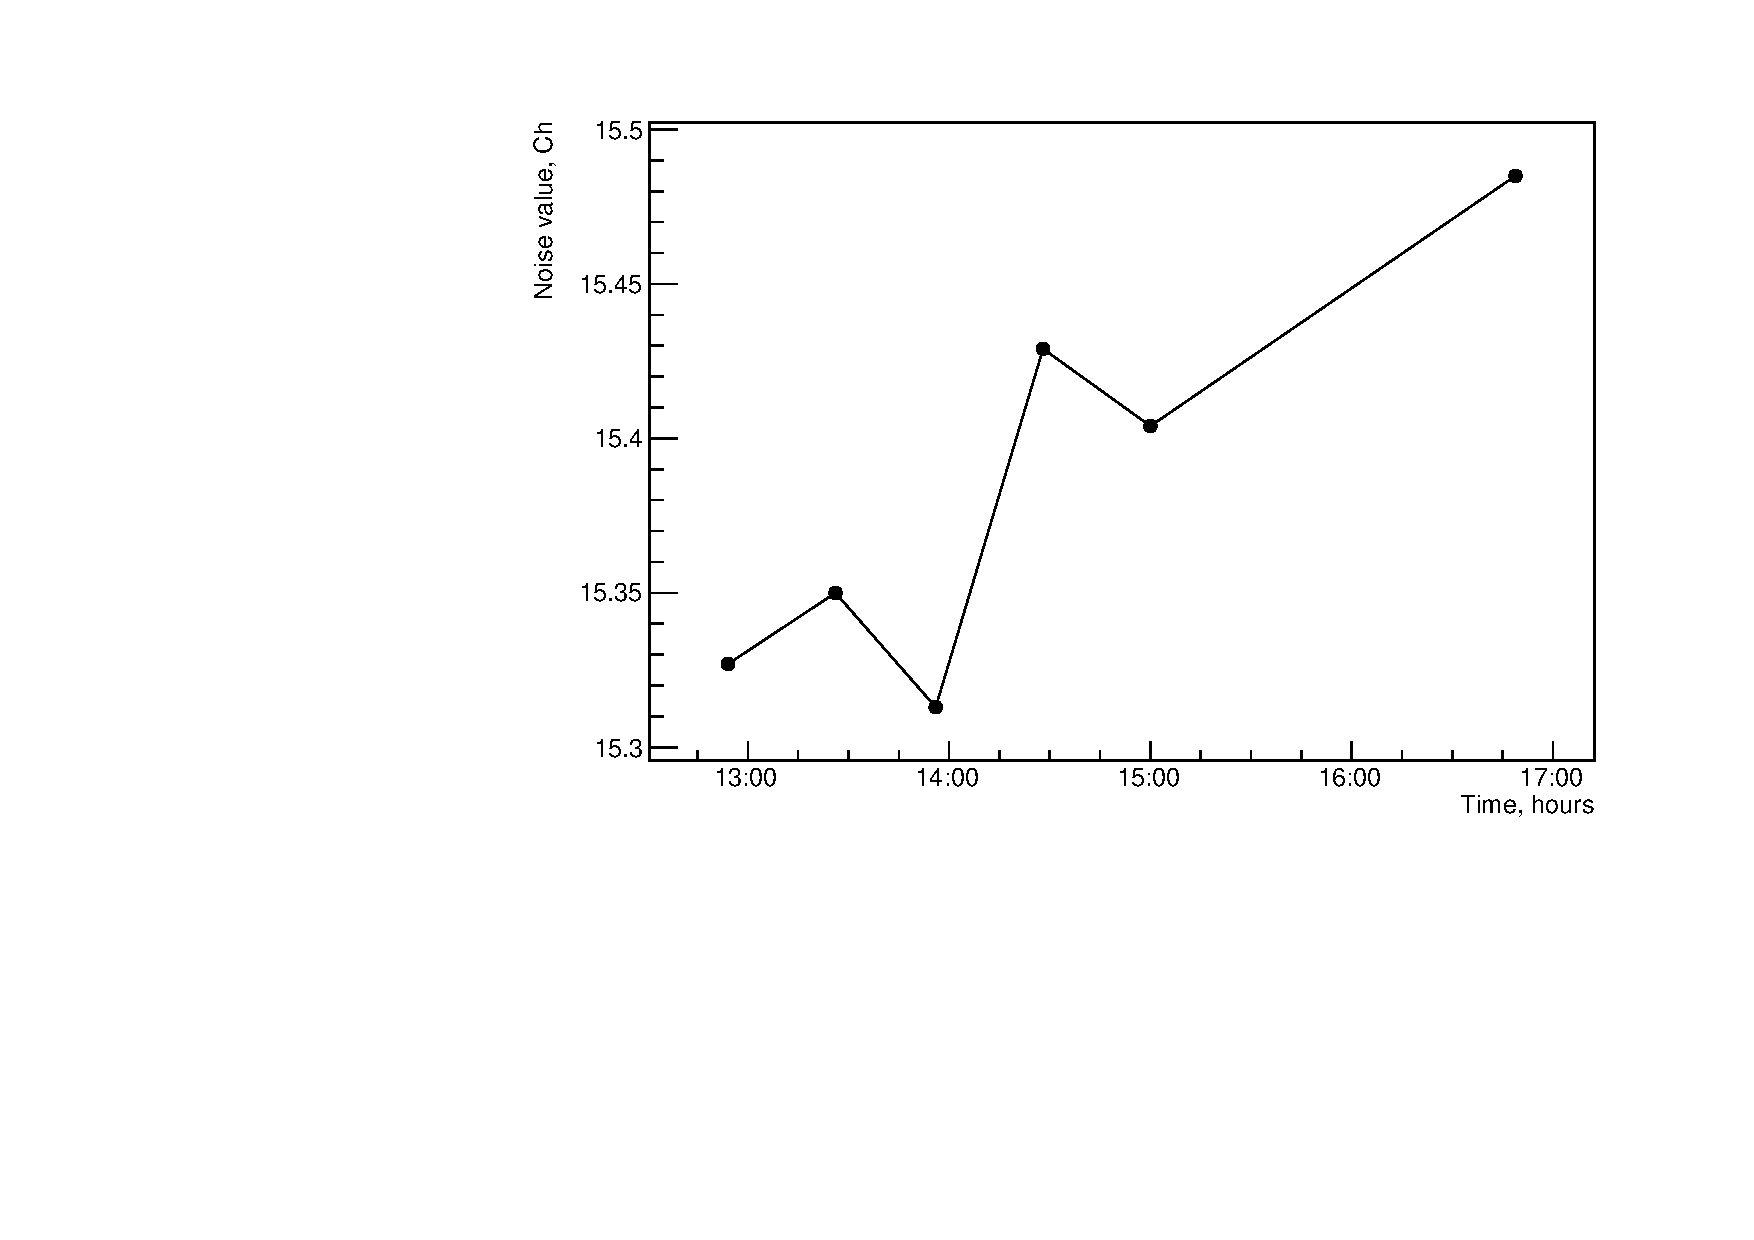
\includegraphics[width=1\linewidth]{img/Noise_time_drift.pdf}
		\caption{Уровень шумов}
	\end{subfigure}%
	\begin{subfigure}{.5\textwidth}
		\centering
		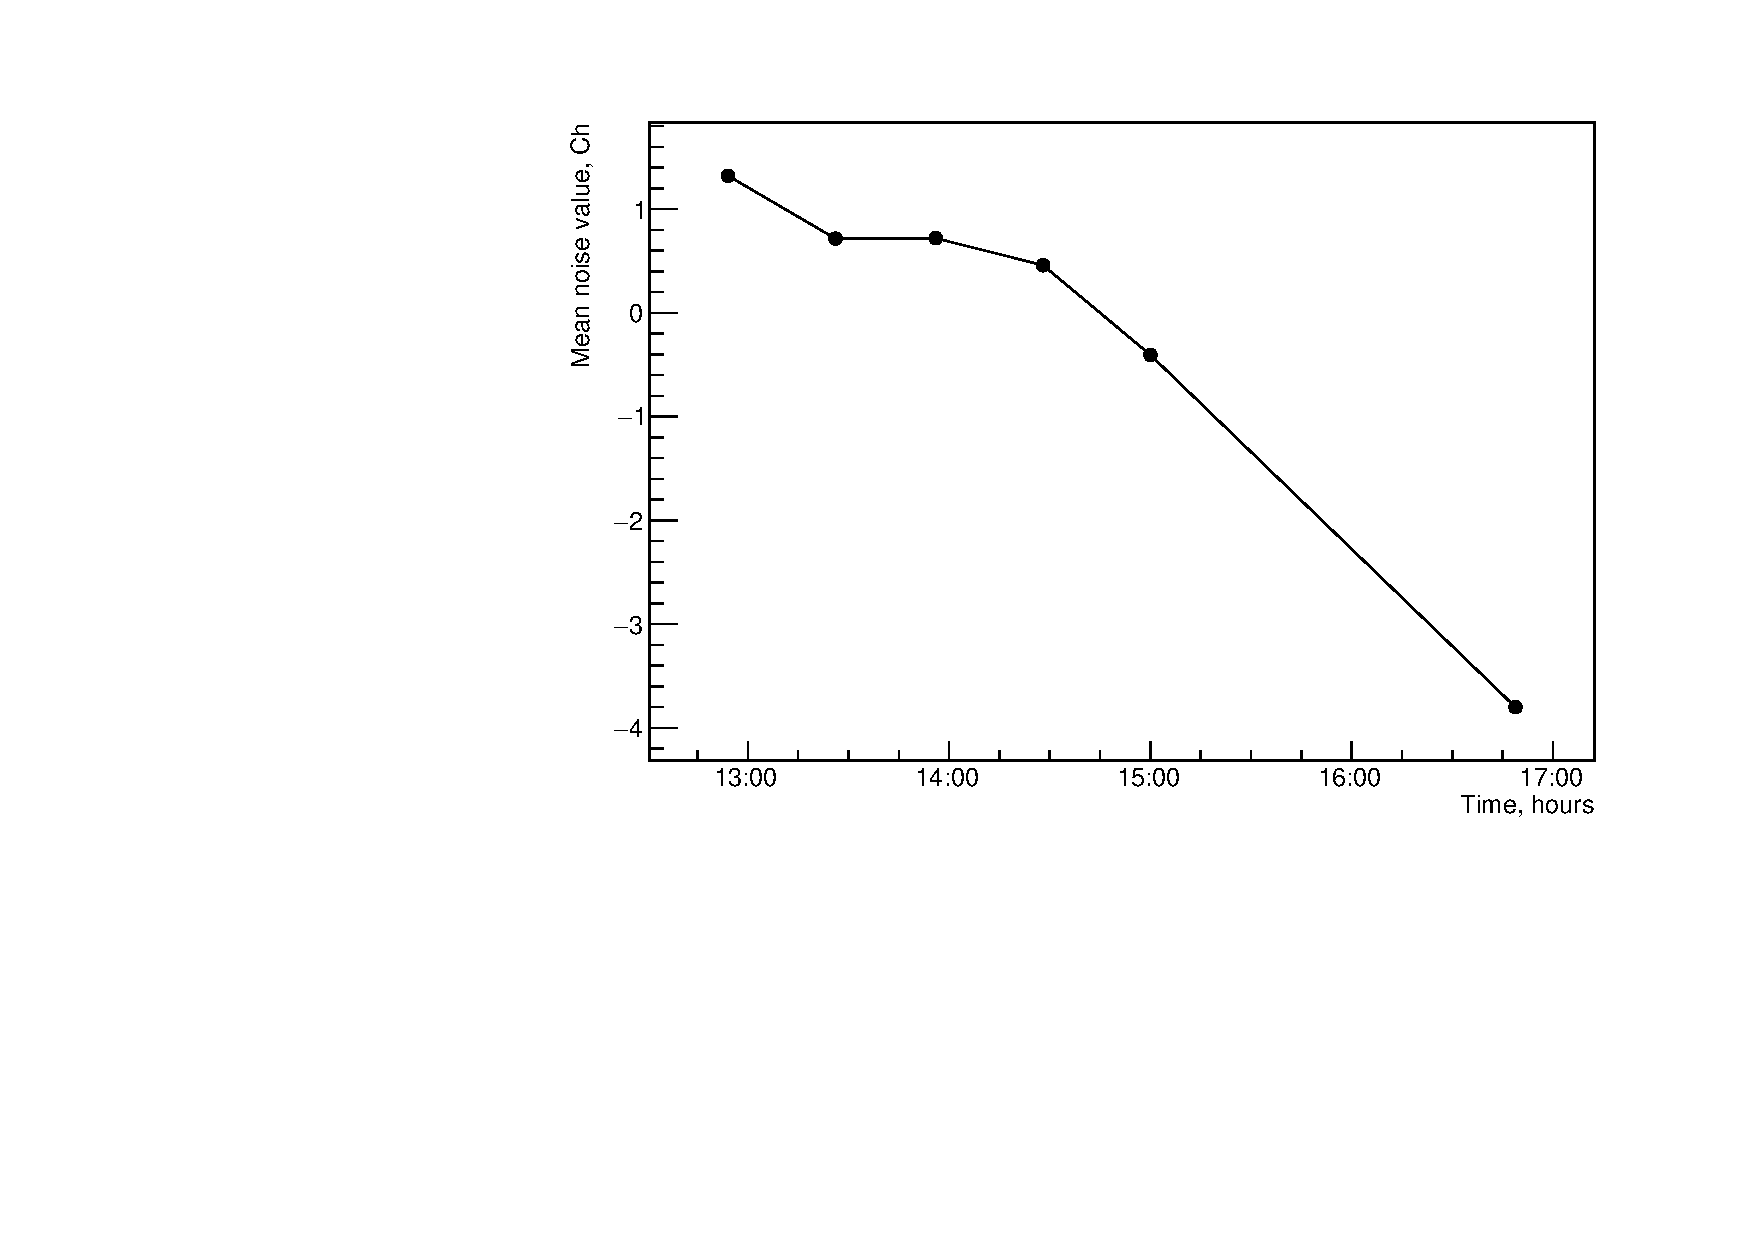
\includegraphics[width=1\linewidth]{img/Mean_time_drift.pdf}
		\caption{Среднее значение шума}
	\end{subfigure}
	\caption{Временной дрейф параметров шумовых событий: уровня шума и среднего значения шума. Каждая точка - среднее по $3\cdot10^7$ значений. В обоих случаях наблюдается линейный тренд.}
	\label{fig:Noise_gr}
\end{figure}
Относительное изменение уровня шума за 4 часа составило $0.01~\sigma$, а дрейф среднего значения -- $0.33~\sigma$. Установившееся значение уровня шумов скорее всего зависит от температурного дрейфа электроники. Это является отдельной довольно обширной темой и в данной работе рассматриваться не будет. Однако, необходимы дополнительные долговременные эксперименты, которые смогут показать, каков максимально достижимый уровень шумов системы и насколько сдвигаются нулевые значения АЦП. Тем не менее, промежуточные результаты показали, что для <<Лазерного поляриметра>> это не является критичным.  
\section{Определение коэффициента усиления}
При исследовании новой модели детектора необходимо различными методами проверить правильность работы, как ускоряющей структуры, так и вычитывающей электроники. Это можно сделать путём измерения коэффициента усиления детектора. 
%Стоит отметить, что зарегистрировать ионизацию первичной частицы достаточно сложно ввиду малого количества заряда. Для этого необходимы высокочувствительные АЦП. Однако, при использовании 
Коэффициент усиления в данной работе определяется как отношение зарегистрированного считывающей структурой заряда кластера к количеству частиц первичной ионизации, образованных в индукционном промежутке. 
Количество частиц первичной ионизации найдем, используя средние ионизационные потери и количество энергии, необходимое для образования ион--электронной пары. Известно, что потери энергии электронов в тонких слоях описываются модифицированной формулой Бете-Блоха:
\begin{equation}
\cfrac{dE}{dx} = \cfrac{2\pi N_0 e^4 Z\rho}{m_e c^2 \beta^2 A}\biggl[ln \bigg(\cfrac{ m_ec^2T\beta^2\gamma^2}{2I^2}\bigg) + f_{corr}(\beta)\biggr],
\label{eq:Bethe_Bloch}
\end{equation}
где $N_0$ -- число Авогадро, $e$ -- элементарный электрический заряд, $m_e$ -- масса электрона, $c$ -- скорость света, $\beta = v/c$ -- отношение скорости частицы к скорости света, $Z$ -- зарядовое число, $A$ -- массовое число, $\rho$ -- плотность вещества, $T$ -- кинетическая энергия электронов, $I$ -- энергия образования ион--электронной пары, $f_{coor}(\beta)$ -- функция, которая содержит поправки в случае $\beta \sim 1$. Параметры $A,Z,\rho$ относятся к веществу--радиатору т.е. к газовой смеси, которой заполнен детектор.
\par Вычисление показало, что средние потери энергии электронов с энергией $2.2~\MeV$ составляют $2.5~\keV/$см. Энергия образования одной ион--электронной пары в аргоне есть $26\eV$. Размер дрейфового промежутка -- 3 мм. Количество первичных электронов:
\begin{equation}
	N_e = \frac{dE/dx~\Delta x}{W} =\frac {2400~\eV/cm \cdot 0.3~cm}{26~\eV} = 28
\end{equation}
Зная средний заряд кластера $\langle Q\rangle$, можно определить коэффициент усиления системы GEM: 
\begin{equation}
K = \frac{\langle Q\rangle}{\langle N_e \ W},
\end{equation}
где $I = 26~\eV$ -- средняя энергия образования ион-электронной пары в аргоне. 
\par Такой метод определения коэффициента усиления имеет один недостаток: в эксперименте определить средний заряд кластера достаточно трудно т.к. существуют ограничения электроники на максимальное измеренное значение. Более того, средний заряд кластера имеет распределение Ландау, параметром которого является наиболее вероятный заряд кластера. Поэтому вместо средних ионизационных потерь необходимо рассчитывать наиболее вероятные. Выражение для них можно записать следующим образом:
\begin{equation}
\Delta_p = \xi\biggl[ln \bigg(\cfrac{ m_ec^2T\beta^2\gamma^2}{2I^2}\bigg) + ln\bigg(\frac{\xi}{I}\bigg) + j - \beta^2 \biggr],
\label{eq:MP_energy_loss}
\end{equation}
где $j=0.2$, а параметр $\xi$ задается формулой:
\begin{equation}
\xi = 2\pi r_0^2 N_A m_ec^2\frac{Z}{A} \frac{\rho x} {\beta^2}, 
\end{equation}
где $r_0$ -- классический радиус электрона, $N_A$ -- число Авогадро. Оценка наиболее вероятных потерь в дрейфовом промежутке дает значение  $\Delta_p = 685~\eV$, а наиболее вероятное количество электронов $[N_e] = 26$, что на самом деле довольно близко к среднему значению.
%https://arxiv.org/pdf/1110.6761.pdf 
\subsection{Постановка эксперимента}
Для определения коэффициента усиления детектор облучался $2.2~\MeV$ электронами источника $Sr-90$, который располагался на герметичном кожухе детектора. Т.к. энергии электронов не хватало, чтобы пройти сквозь детектор, организация внешнего триггера по схеме совпадений не представлялась возможной. Поэтому запуск детектора проводился в автоматическом режиме. Первичная ионизация из дрейфового промежутка попадает в ускоряющую структуру, где происходит образование электронных лавин и инжекция заряда в индукционный промежуток. Далее заряд кластеров регистрируется считывающей структурой. 
\begin{figure}[H]
	\centering
	\begin{subfigure}{.5\textwidth}
		\centering
		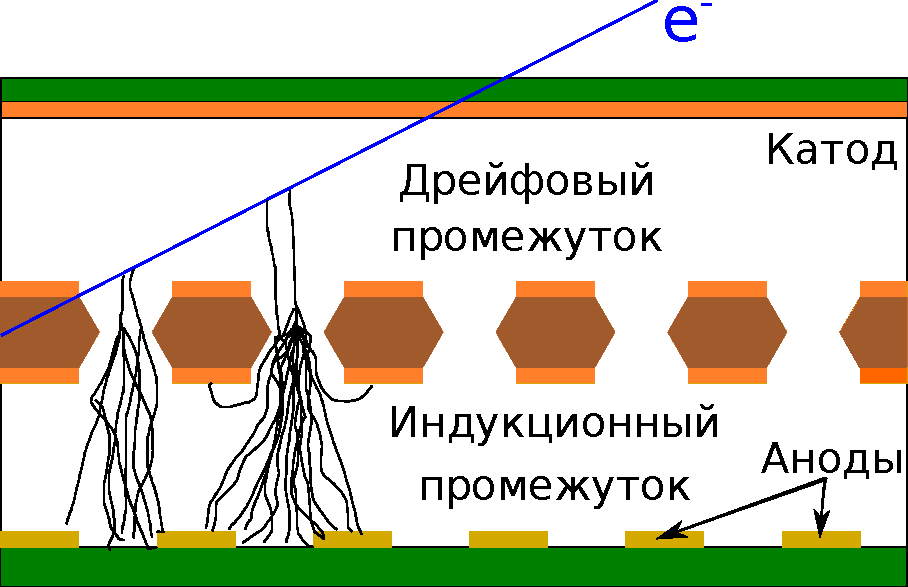
\includegraphics[height = 4 cm, width= 6cm]{img/GEM_scheme.pdf}
		\caption{\centering {Процесс образования лавины от первичной ионизирующей частицы}}
		\label{fig:ionization_scheme}
	\end{subfigure}%
	\begin{subfigure}{.5\textwidth}
		\centering
		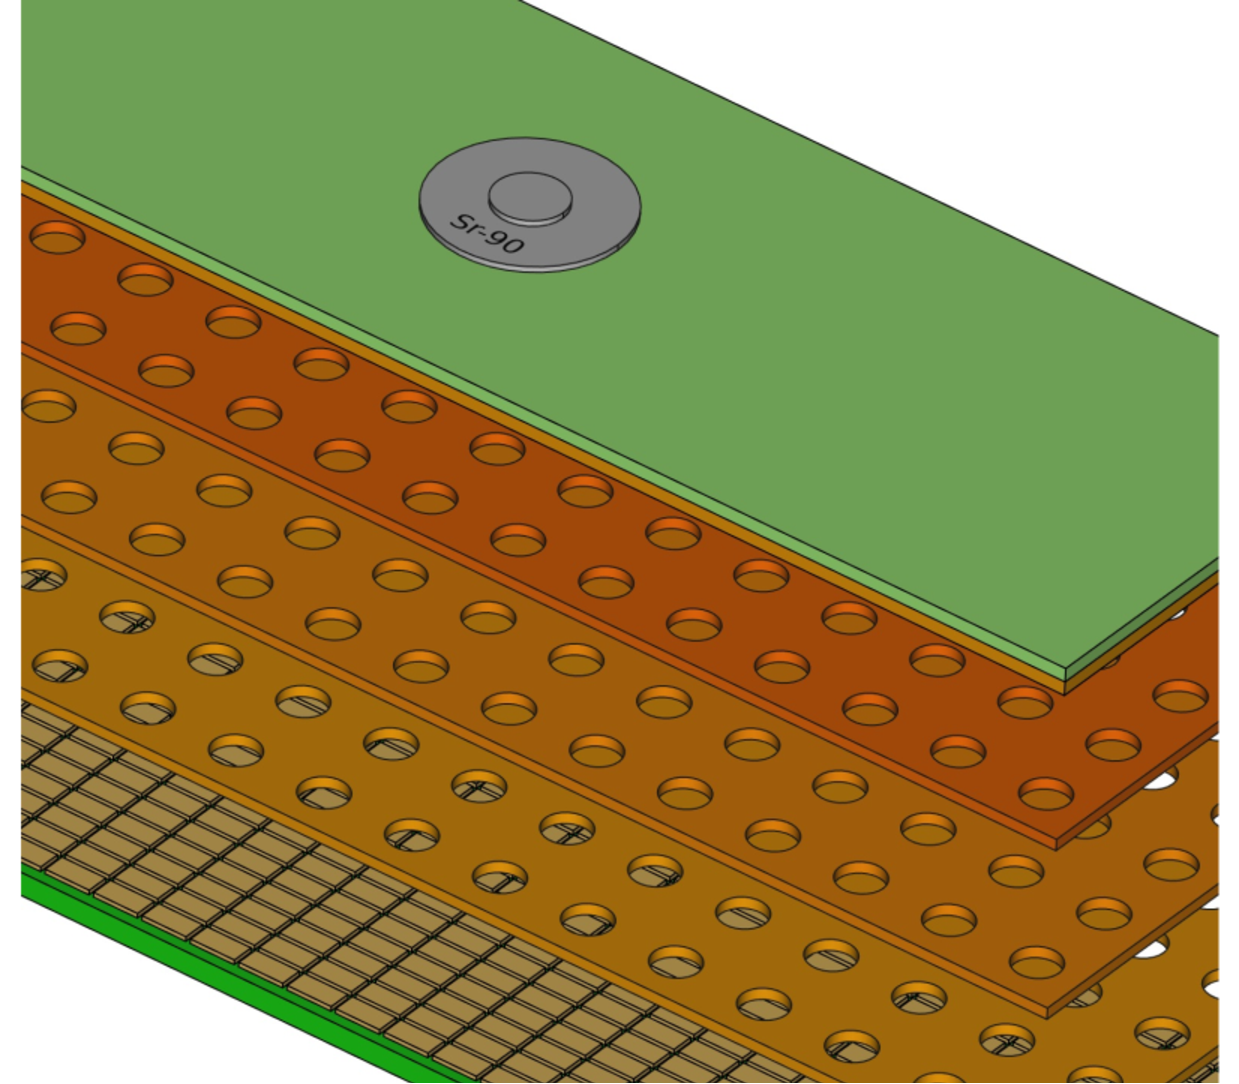
\includegraphics[height = 4 cm, width= 5.8cm]{img/GEM_Sr_source.pdf}
		\caption{\centering {Расположение источника относительно ускоряющей структуры}}
		\label{fig:det_scheme+sr90}
	\end{subfigure}
	\caption{Схема проведения эксперимента по определению коэффициента усиления детектора.}
	\label{fig:ampl_exp}
\end{figure}

\subsection{Обработка и анализ полученных данных}

\subsection{Результаты}
\section{Определение эффективности регистрации}
\section{Определение пространственного разрешение}